\section{The individual-cover bound and the equality}
\label{sec:lower-bound}

All ingredients are now available. We apply the continuous bundle
embedding of \Cref{prop:comparison-bundle} to the packet maps, use
\Cref{thm:torus-compression}, and reconstruct one finite target complex
for the full orbit cover. The proof keeps the rank margin and the
cover-order saving in the same strict parameter budget.

\subsection{A comparison bound controls every cover rate}

We use comparison bounds in the sense of
\Cref{eq:comparison-bound}.  In particular, traces on $A$ are
normalized and their matrix extensions use the unnormalized
matrix trace.

\Needspace{6\baselineskip}
\begin{theorem}
\label{thm:cover-bound}
Let $h$ be a minimal homeomorphism of an infinite compact
metrizable space $X$, and let $A=C(X)\rtimes_h\Z$.
For every finite comparison bound $r$ for $A$ and every finite
open cover $\mathcal U$ of $X$,
\[
 \lim_{k\to\infty}\frac{D(\mathcal U^{[0,k)})}{k}\le2r.
\]
\end{theorem}

\begin{proof}
Suppose, to the contrary, that a cover has rate $d>2r$.
By \Cref{eq:finite-cover-rate}, $d$ is finite.  We choose the
parameters so that the bundle embedding and the covering-order
decrease have simultaneous strict margins.

\paragraph{Choice of parameters.}
First choose an integer $p\ge1$ such that, for $t=2p+1$,
\[
 \frac{pd}{t+1}>r.
\]
This is possible because $p/(2p+2)\to1/2$.  Set
$c_0=d/(t+1)>0$, and choose $0<a<1/16$ so small that
\begin{equation}
\label{eq:cover-a-choice}
 (1-11a)pc_0>r.
\end{equation}
Choose an integer $H_0\ge2$ so large that
\begin{equation}
\label{eq:cover-height-choice}
 \frac{2-10a}{H_0-1}<2a,
 \qquad
 \frac{d}{H_0}<\frac{ac_0}{32}.
\end{equation}
Next choose $b_0>0$ satisfying
\begin{equation}
\label{eq:cover-bad-choice}
 b_0<\frac{a}{32},
 \qquad b_0(d+c_0)<\frac{ac_0}{64}.
\end{equation}
These choices precede the choice of $k$.

For $m=m_k$, put
\begin{equation}
\label{eq:cover-g-r-choice}
 g=\left\lfloor\frac{m+1}{t+1}\right\rfloor,
 \qquad R=\lfloor(2-10a)pg\rfloor.
\end{equation}
As $k\to\infty$,
\[
 \frac{m}{k}\longrightarrow d,
 \qquad \frac{g}{k}\longrightarrow c_0,
 \qquad \frac{R-pg}{k}\longrightarrow(1-10a)pc_0>r.
\]
For every $k$ with $g>0$, the first inequality in
\Cref{eq:cover-height-choice} gives
\begin{align}
\label{eq:cover-comparison-parameters}
 \frac{RH_0}{pg(H_0-1)}+2(a+b_0)
 &\le 2-8a+\frac{2-10a}{H_0-1}+2b_0<2.
\end{align}
The strict inequality follows from $b_0<a/32$.

The cover construction below treats each interval of length $kH_0$
with $H_0-1$ reconstructed length-$k$ blocks and two unchanged edge
blocks.  Their nerve factors have total dimension at most $(H_0+1)m$
before counting the missing colors.  An alternative description uses
$H_0$ unchanged blocks.  Joining the two descriptions can add at most
$H_0m+1$ dimensions, and this extra cost will occur on at most a
$b_0$ fraction of the intervals.  Each interval has $(H_0-1)g$ slots.
Compression puts at least an $a/8$ fraction of all slots on the boundary;
discarding those in these exceptional intervals loses at most a $b_0$
fraction of all slots.  The retained boundary slots therefore reduce the
dimension bound by at least $(a/8-b_0)(H_0-1)g$ per interval on average.
These three contributions give the prospective cover-rate bound
\begin{equation}
\label{eq:cover-rate-budget}
 E_k=
 \frac{(H_0+1)m+b_0(H_0m+1)
       -(a/8-b_0)(H_0-1)g}{kH_0}.
\end{equation}
Its limiting excess over $d$ is
\begin{align*}
 \lim_{k\to\infty}(E_k-d)
 &=\frac d{H_0}
   -\frac a8\left(1-\frac1{H_0}\right)c_0
   +b_0\left(d+\left(1-\frac1{H_0}\right)c_0\right)\\
 &<\frac{ac_0}{32}-\frac{ac_0}{16}
       +\frac{ac_0}{64}
   =-\frac{ac_0}{64}.
\end{align*}
Here we used $H_0\ge2$ and
\Cref{eq:cover-height-choice,eq:cover-bad-choice}.
We may therefore fix $k$ large enough that $g\ge1$ and
\begin{equation}
\label{eq:cover-final-parameters}
 \frac{R-pg}{k}>r,
 \qquad E_k<d.
\end{equation}
In particular $R>pg$.  All of $p,t,a,H_0,b_0,k,m,g,R$ are now
fixed.  Put $e=kH_0$.

\paragraph{The subordinate functions and their compression.}
Apply \Cref{lem:colored-subordinate-nerve} to
$\mathcal U^{[0,k)}$, and write $\phi:X\to S$ for the resulting
map.  For every vertex $v$ of $S$, fix members
$U(v,s)\in\mathcal U$, $0\le s<k$, such that
\begin{equation}
\label{eq:time-vertex-subordination}
 \lambda_v(\phi(x))>0
 \quad\Longrightarrow\quad
 h^s x\in U(v,s)\quad(0\le s<k).
\end{equation}
These members come from the assigned element of the orbit join.
Use \Cref{lem:packet-reconstruction} to define
\[
 F_j=\mathcal F_j\circ\phi:X\longrightarrow C_t,
 \qquad 1\le j\le g.
\]

The estimates in
\Cref{eq:cover-comparison-parameters,eq:cover-final-parameters}
allow us to use
\Cref{lem:uniform-block-allocation,prop:comparison-bundle}.
Keep the open labeled regions $O_i$, $0\le i<k$, and the
continuous weight $w:X\to[0,1]$ supplied there.  For some $J_0$,
their uniform frequency property is
\begin{equation}
\label{eq:cover-macro-frequency}
 \#\{0\le q<J:w(h^{qe}y)<1\}\le b_0J
 \qquad(y\in X,\ J\ge J_0).
\end{equation}
Choose and fix one $J\ge J_0$ sufficiently large for
\Cref{prop:comparison-bundle}, and put
\[
 N=eJ,\qquad n=J(H_0-1)g.
\]
The proposition gives a continuous map
$f:X\to C_t^n$ whose coordinates are indexed by
\[
 (q,D,j),\qquad
 0\le q<J,\quad 0\le D<H_0-1,\quad 1\le j\le g.
\]
Whenever $w(h^{qe}y)>0$ and $h^{qe}y\in O_i$, these coordinates
satisfy
\begin{equation}
\label{eq:cover-aligned-f}
 f_{q,D,j}(y)=F_j(h^{qe+i+Dk}y).
\end{equation}
Moreover the rank-$pn$ torus bundle over the sparse test locus
for $f$ embeds in a trivial bundle of rank strictly less than
$2pn$.

By \Cref{thm:torus-compression}, for arbitrarily large integers
$u$ there is a continuous map
\[
 G:X^u\longrightarrow C_t^{un}
\]
with at least $(a/8)un$ boundary slots at every point, agreeing
with each original slot of $f^{\times u}$ whenever that slot is on its
boundary.  Pull it back along the map of actual orbit starts
\[
 \iota_u:X\longrightarrow X^u,
 \qquad
 \iota_u(x)=(x,h^Nx,\ldots,h^{(u-1)N}x).
\]
Denote the resulting slot functions by
$\widetilde F_{b,q,D,j}(x)$, with $0\le b<u$ and the other
indices as above.  They retain the boundary agreement and the
pointwise count
\begin{equation}
\label{eq:cover-total-successes}
 \#\{(b,q,D,j):\widetilde F_{b,q,D,j}(x)\in\partial C_t\}
 \ge\frac a8un.
\end{equation}

\paragraph{Aligned and fallback descriptions.}
The orbit pullback has provided the boundary slots. We next encode their
reconstructed nerve points in a fixed finite polyhedron, including the
points where the alignment label is unavailable.
Fix one of these integers $u$.  The $uJ$ successive
macro-intervals have starting times
\[
 T_{b,q}=bN+qe,\qquad 0\le b<u,\quad 0\le q<J.
\]
On the open set where $w(h^{T_{b,q}}x)>0$, let $i$ be the unique
label with $h^{T_{b,q}}x\in O_i$.  The label is locally constant
there.  For each $0\le D<H_0-1$, use
\Cref{lem:packet-reconstruction} at the original point
\[
 \phi(h^{T_{b,q}+i+Dk}x)\in S
\]
with replacements $\widetilde F_{b,q,D,j}(x)$, $1\le j\le g$.
\Cref{eq:packet-boundary-condition} holds by
\Cref{eq:cover-aligned-f} and the boundary agreement of $G$.
Let the resulting continuous map on this open set be
$\psi_{b,q,D}(x)\in S$.  It has exact vertex subordination to
the displayed original point.  If $s_{b,q,D}(x)$ of these $g$
replacement slots are on their boundaries, then
\begin{equation}
\label{eq:cover-updated-carrier}
 \dim\operatorname{car}(\psi_{b,q,D}(x))
 \le m-s_{b,q,D}(x).
\end{equation}

Use the finite polyhedra
\[
 \mathcal A=\coprod_{i=0}^{k-1}S^{H_0+1},
 \qquad \mathcal B=S^{H_0},
 \qquad \mathcal J=\mathcal A*\mathcal B.
\]
The aligned point in the copy of $\mathcal A$ labeled $i$ is
\begin{equation}
\label{eq:cover-aligned-description}
 A_{b,q}(x)=
 \bigl(i;\phi(h^{T_{b,q}}x),
       \psi_{b,q,0}(x),\ldots,\psi_{b,q,H_0-2}(x),
       \phi(h^{T_{b,q}+e-k}x)\bigr).
\end{equation}
Its first and last factors retain the two edge blocks.
The fallback point, defined on all of $X$, is
\begin{equation}
\label{eq:cover-fallback-description}
 B_{b,q}(x)=
 \bigl(\phi(h^{T_{b,q}}x),\phi(h^{T_{b,q}+k}x),
       \ldots,\phi(h^{T_{b,q}+(H_0-1)k}x)\bigr).
\end{equation}
In the join, give the aligned branch weight $w(h^{T_{b,q}}x)$
and the fallback branch weight $1-w(h^{T_{b,q}}x)$.
Although the aligned coordinates are needed only where their
weight is positive, this defines a continuous map to
$\mathcal J$.  To see this directly, embed the finitely many
copies of the product polyhedra in Euclidean space.  Every
aligned coordinate, including the label indicator, is bounded
and continuous where its weight is positive; multiplying it by
that weight and setting it to zero at weight zero is continuous.
These are the usual coordinates for the join.  Taking all the
macro-intervals gives a continuous map
\begin{equation}
\label{eq:cover-total-description}
 \Phi_u:X\longrightarrow\mathcal K_u:=\mathcal J^{uJ}.
\end{equation}

\paragraph{The descriptions retain the entire orbit cover.}
We give a finite open cover of $\mathcal K_u$ whose pullback
under $\Phi_u$ refines $\mathcal U^{[0,uN)}$.
In one join factor let $\omega$ be the weight of its aligned
branch.  For an aligned label $i$, a factor index
$0\le\ell\le H_0$, and a vertex $v$ of $S$, the function
\[
 \alpha_{i,\ell,v}
   =\omega\,\mathbf 1_{\{\text{aligned label }i\}}
       \lambda_v(a_\ell)
\]
is continuous on the join when extended by zero where the
aligned branch is collapsed.  Similarly, for $0\le\ell<H_0$,
\[
 \beta_{\ell,v}=(1-\omega)\lambda_v(b_\ell)
\]
is continuous, with value zero where the fallback branch is
collapsed.  Here $a_\ell$ and $b_\ell$ denote the simplicial
factors in the two descriptions.

Form open sets of two kinds: choose a label $i$ and one vertex
in each aligned factor, requiring all the corresponding
$\alpha$'s to be positive; or choose one vertex in each fallback
factor, requiring all the corresponding $\beta$'s to be
positive.  These finitely many sets cover $\mathcal J$, because
at every point some branch has positive weight and every
simplicial factor has a positive vertex coordinate.  Their
products form a finite open cover of $\mathcal K_u$.

Fix one member of this product cover.  In each macro-interval
it fixes a branch, its label when aligned, and one positive
vertex per simplicial factor.  Under $\Phi_u$, an updated
factor with positive vertex $v$ has that same vertex positive
in its original point, by \Cref{lem:packet-reconstruction}.
Thus \Cref{eq:time-vertex-subordination} applies to every
chosen factor, updated or unchanged, and gives fixed members
of $\mathcal U$ along its length-$k$ orbit block.

For a fallback description the block starts relative to the
macro-interval are $0,k,\ldots,(H_0-1)k$, so these blocks cover
$[0,e)$.  For an aligned description the starts are
\[
 0,\quad i+Dk\ (0\le D<H_0-1),\quad e-k.
\]
Their length-$k$ intervals also cover $[0,e)$: the middle
blocks cover $[i,i+(H_0-1)k)$, the first edge covers the
beginning since $0\le i<k$, and the last edge covers the end
since $i+(H_0-1)k\ge e-k$.  All of these blocks lie within the
macro-interval.  For each time in it, choose one of its covering
blocks.  The fixed vertex and the offset within that block
select one fixed member of $\mathcal U$ by
\Cref{eq:time-vertex-subordination}.

Figure~\ref{fig:block-allocation} shows the two edge overlaps and the
fallback partition for one macro-interval.
\begin{figure}[tbp]
  \centering
  \begingroup
  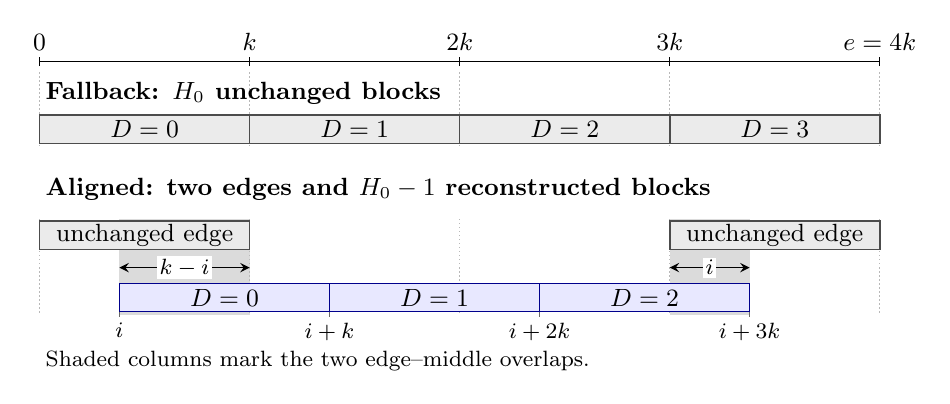
\begin{tikzpicture}[
    x=.22\linewidth,y=8mm,
    font=\small,
    every node/.style={inner sep=2pt},
    original/.style={draw=black!70,fill=black!8,line width=.55pt},
    reconstructed/.style={draw=blue!55!black,fill=blue!9,line width=.55pt},
    overlap/.style={fill=black!14,draw=none},
    guide/.style={draw=black!28,densely dotted,line width=.45pt}
  ]
    \def\blockoffset{.38}

    \draw[line width=.55pt] (0,5.15) -- (4,5.15);
    \foreach \x/\lab in {0/0,1/k,2/2k,3/3k,4/{e=4k}} {
      \draw (\x,5.08) -- (\x,5.22);
      \node[above] at (\x,5.23) {$\lab$};
      \draw[guide] (\x,4.98) -- (\x,3.78);
    }

    \node[anchor=west,font=\small\bfseries] at (0,4.65)
      {Fallback: $H_0$ unchanged blocks};
    \foreach \D in {0,1,2,3} {
      \draw[original] (\D,3.85) rectangle ({\D+1},4.30);
      \node at ({\D+.5},4.075) {$D=\D$};
    }

    \node[anchor=west,font=\small\bfseries] at (0,3.12)
      {Aligned: two edges and $H_0-1$ reconstructed blocks};

    \path[overlap] (\blockoffset,1.13) rectangle (1,2.65);
    \path[overlap] (3,1.13) rectangle ({3+\blockoffset},2.65);
    \foreach \x in {0,1,2,3,4} {
      \draw[guide] (\x,2.65) -- (\x,1.13);
    }
    \draw[original] (0,2.17) rectangle (1,2.62);
    \draw[original] (3,2.17) rectangle (4,2.62);
    \node at (.5,2.395) {unchanged edge};
    \node at (3.5,2.395) {unchanged edge};

    \foreach \D in {0,1,2} {
      \draw[reconstructed]
        ({\blockoffset+\D},1.18)
        rectangle ({\blockoffset+\D+1},1.63);
      \node at ({\blockoffset+\D+.5},1.405) {$D=\D$};
    }
    \foreach \D/\lab in {0/i,1/{i+k},2/{i+2k},3/{i+3k}} {
      \draw[black!60] ({\blockoffset+\D},1.10)
        -- ({\blockoffset+\D},1.18);
      \node[below,font=\footnotesize] at ({\blockoffset+\D},1.10)
        {$\lab$};
    }

    \draw[<->,>=stealth,line width=.5pt]
      (\blockoffset,1.88) -- (1,1.88)
      node[midway,font=\footnotesize,fill=white,inner sep=1pt] {$k-i$};
    \draw[<->,>=stealth,line width=.5pt]
      (3,1.88) -- ({3+\blockoffset},1.88)
      node[midway,font=\footnotesize,fill=white,inner sep=1pt] {$i$};
    \node[anchor=west,font=\footnotesize] at (0,.40)
      {Shaded columns mark the two edge--middle overlaps.};
  \end{tikzpicture}
  \endgroup
  \caption{Aligned and fallback coverage of one macro-interval, translated
    to $[0,e)$. The schematic uses $H_0=4$ and $0<i<k$; every bar denotes
    a half-open interval of length $k$. In general, $e=kH_0$, and the
    middle blocks, with starts $i+Dk$ for $0\le D<H_0-1$, cover
    $[i,e-k+i)$. The unchanged edges $[0,k)$ and $[e-k,e)$ complete the
    coverage. Their overlaps with the middle union are $[i,k)$ and
    $[e-k,e-k+i)$, of lengths $k-i$ and $i$. All blocks lie in $[0,e)$.
    The fallback blocks partition $[0,e)$; at $i=0$, the first middle
    block duplicates the left edge.}
  \label{fig:block-allocation}
\end{figure}


Doing this in all $uJ$ macro-intervals shows that the whole
preimage of the chosen target open set is contained in one
fixed member of $\mathcal U^{[0,uN)}$.  The assertion is about
the whole preimage; no injectivity of $\Phi_u$ is required.

\paragraph{A finite subcomplex of smaller dimension.}
The target description now retains every member of the orbit-cover
information. It remains to bound the dimension of a single subcomplex
containing its image; this is where the pointwise boundary count produces
the strict decrease in cover rate.
Equip the products of copies of $S$ with their product cells,
the joins with the joins of those cells and their endpoint
cells, and $\mathcal K_u$ with the resulting product cell
structure.  These are finite polytopal complexes and admit
compatible simplicial subdivisions.  In a join, the carrier
dimension is the dimension of the retained branch at an
endpoint and is the sum of the two carrier dimensions plus
one when both weights are positive.  Product carrier
dimensions add.

Call a macro-interval good at $x$ if $w(h^{T_{b,q}}x)=1$,
and bad otherwise.  Apply \Cref{eq:cover-macro-frequency}
to $y=h^{bN}x$ in each of the $u$ windows.  The number
$B_u(x)$ of bad macro-intervals satisfies
\begin{equation}
\label{eq:cover-bad-count}
 B_u(x)\le b_0uJ.
\end{equation}
Each macro-interval has $(H_0-1)g$ replacement slots.
Consequently at most $b_0un$ of the boundary slots in
\Cref{eq:cover-total-successes} can belong to bad intervals.
If $S_u^{\mathrm{good}}(x)$ is the number of boundary slots
in good intervals, then
\begin{equation}
\label{eq:cover-good-successes}
 S_u^{\mathrm{good}}(x)\ge(a/8-b_0)un.
\end{equation}

At a good interval the join is at its aligned endpoint.
The two unchanged edge factors cost at most $2m$, and
\Cref{eq:cover-updated-carrier} bounds the other factors.
Thus its carrier dimension is at most
\[
 (H_0+1)m-\sum_{D=0}^{H_0-2}s_{b,q,D}(x).
\]
At a bad interval we may ignore all successful slots.  Its
carrier dimension is at most $(2H_0+1)m+1$: this bounds
the sum of the aligned and fallback dimensions plus one,
and also bounds the fallback endpoint.  Using
\Cref{eq:cover-bad-count,eq:cover-good-successes},
the carrier dimension of $\Phi_u(x)$ is therefore at most
\begin{align*}
 &(uJ-B_u(x))(H_0+1)m
   +B_u(x)((2H_0+1)m+1)-S_u^{\mathrm{good}}(x)\\
 &\qquad\le uJ\bigl((H_0+1)m+b_0(H_0m+1)\bigr)
                 -(a/8-b_0)un\\
 &\qquad= uJ\bigl((H_0+1)m+b_0(H_0m+1)
                   -(a/8-b_0)(H_0-1)g\bigr)
   =uNE_k.
\end{align*}
It follows that $\Phi_u(X)$ lies in the finite subcomplex
consisting of all cells of dimension at most
$\lfloor uNE_k\rfloor$, together with their faces.  In
particular this is an actual subcomplex dimension bound,
not a bound on dimensions of fibers or on a varying family
of images.

Restrict the finite target open cover constructed above
to this subcomplex, triangulate it compatibly, and apply
\Cref{lem:polyhedral-refinement}.  We obtain
\[
 D(\mathcal U^{[0,uN)})\le\lfloor uNE_k\rfloor,
 \qquad
 \frac{D(\mathcal U^{[0,uN)})}{uN}\le E_k<d.
\]
By \Cref{eq:finite-cover-rate}, $d$ is the infimum of all normalized
cover orders, so even one such $u$ gives a contradiction.  This proves
the theorem.
\end{proof}

\subsection{The extended-real equality}

\begin{proof}[Proof of \Cref{thm:main}]
Put $A=C(X)\rtimes_h\Z$.
Minimality and infinitude imply that $h$ is free: a periodic
orbit would be a finite nonempty closed invariant subset of
$X$, and hence all of $X$.  Niu's upper bound therefore gives
\begin{equation}
\label{eq:final-niu-upper-bound}
 \rc(C(X)\rtimes_h\Z)\le\frac12\mdim(X,h)
\end{equation}
in the extended nonnegative reals
\cite[Theorem~5.6]{Niu2024}.

Let $\mathcal R$ be the set of finite comparison bounds in
the definition of the radius of comparison.  For every
$r\in\mathcal R$, \Cref{thm:cover-bound} and the supremum
over all finite open covers give
\[
 \mdim(X,h)\le2r.
\]
If $\mathcal R$ is nonempty, taking its infimum yields
$\mdim(X,h)/2\le\rc(A)$.  This passage does not require
the infimum itself to belong to $\mathcal R$.  If
$\mathcal R$ is empty, the same lower inequality holds
because $\rc(A)=\infty$ by definition.  Together with
\Cref{eq:final-niu-upper-bound}, this proves the equality.

Explicitly, when $\mdim(X,h)=\infty$,
\Cref{thm:cover-bound} excludes every finite comparison
bound, so $\rc(A)=\infty$.  When $\mdim(X,h)=0$,
\Cref{eq:final-niu-upper-bound} and nonnegativity give
$\rc(A)=0$.  The argument above covers all intervening
finite values with the same trace normalization.
\end{proof}
